% Motor: XeLaTeX. Sesion 17 - material docente UTP.
% Misma estructura docente que la Sesion 16.
\documentclass[aspectratio=169,10pt,c]{beamer}
% Reutiliza sin cambios la identidad visual UTP validada en la Sesion 09.
% Reutiliza sin cambios la identidad visual UTP validada en la Sesion 08.
% Reutiliza sin cambios la identidad visual UTP validada en la Sesion 05.
% La segunda ruta permite compartir los assets comunes sin duplicar binarios.
\input{../../Sesion05/slides/header.tex}
\graphicspath{{../../Sesion05/slides/assets/}}



% assets/ guarda las capturas del curso de Google Skills propias de esta sesion.
\graphicspath{{assets/}{../../Sesion05/slides/assets/}}
% Bloques de código con el mismo estilo que la Sesion 11.
\usepackage{listings}
\lstset{basicstyle=\ttfamily\small,backgroundcolor=\color{utpGrisClaro},
  frame=none,aboveskip=4pt,belowskip=4pt,showstringspaces=false,
  columns=fullflexible,keepspaces=true,breaklines=true,
  xleftmargin=5pt,xrightmargin=5pt,framesep=5pt}


\title{Integración de Servicios Cloud GCP}
\subtitle{Ruta Associate Cloud Engineer: la consola de Google Cloud y Cloud Shell}
\date{Semana 09 - Sesión 17}
\author{Rel Guzman}

\begin{document}

{\setbeamertemplate{footline}{}\maketitle}

% ------------------------------------ Revision: el recorrido por los labs
\begin{frame}{Revisión de la sesión anterior (1/3): el recorrido}
\begin{block}{Qué es}
\small \emph{Recorrido por los labs prácticos de Google Cloud} es la \textbf{actividad 1} de la ruta. No enseña un servicio: enseña a \textbf{usar la plataforma de labs} de Google Skills.
\end{block}
\begin{columns}[T,onlytextwidth]
\column{.48\textwidth}
\begin{exampleblock}{Todo lab funciona igual}
\small
\textbf{1. Comenzar lab:} Google crea un \textbf{proyecto temporal} solo para ti.\par\smallskip
\textbf{2.} Te da un \textbf{usuario y contraseña} de prueba.\par\smallskip
\textbf{3.} Corre un \textbf{temporizador}.\par\smallskip
\textbf{4. Revisar mi progreso} califica cada tarea.\par\smallskip
\textbf{5. Finalizar lab} borra todo.
\end{exampleblock}
\column{.48\textwidth}
\begin{block}{Una comparación}
\small Una \textbf{cabina de Internet}: te dan una PC lista y un tiempo. Al irte, la PC se limpia para el siguiente. No pagas la PC ni rompes nada tuyo.
\end{block}
\begin{alertblock}{Lo mismo, fuera de Google (gratis)}
\small \textbf{Killercoda} y \textbf{Play with Docker}: terminales de práctica en el navegador. \textbf{Microsoft Learn} tiene su \emph{sandbox} de Azure.
\end{alertblock}
\end{columns}
\end{frame}

\begin{frame}{Revisión de la sesión anterior (2/3): lo que muestra}
\begin{block}{Tres ideas de Google Cloud que aparecen en ese lab}
\small Las tres se usan en \textbf{todos} los labs que siguen. Cada una tiene un parecido con algo que ya conoces.
\end{block}
\begin{columns}[T,onlytextwidth]
\column{.31\textwidth}
\begin{exampleblock}{Proyecto}
\small La \textbf{caja} donde vive todo lo que creas. Tiene \textbf{nombre}, \textbf{ID} (único, no cambia) y \textbf{número}.\par\smallskip
\emph{Se parece a:} un \textbf{repositorio} de GitHub o una carpeta de Drive por cada trabajo.
\end{exampleblock}
\column{.31\textwidth}
\begin{exampleblock}{IAM}
\small \textbf{Quién} puede hacer \textbf{qué}. A cada usuario se le da un \textbf{rol}, y el rol trae \textbf{permisos}.\par\smallskip
\emph{Se parece a:} compartir un archivo de Drive como \textbf{lector}, \textbf{comentador} o \textbf{editor}.
\end{exampleblock}
\column{.31\textwidth}
\begin{exampleblock}{APIs}
\small Cada servicio tiene un \textbf{interruptor}. Antes de usarlo se \textbf{habilita} en la \emph{Biblioteca de APIs}.\par\smallskip
\emph{Se parece a:} darle a una app del celular el \textbf{permiso} de cámara antes de usarla.
\end{exampleblock}
\end{columns}
\end{frame}

\begin{frame}{Revisión de la sesión anterior (3/3): pregunta rápida}
\begin{columns}[T,onlytextwidth]
\column{.48\textwidth}
\begin{alertblock}{Lo desactualizado del lab}
\small Sus \textbf{capturas} son de una consola anterior y todavía nombra \textbf{Qwiklabs} y \textbf{Cloud Skills Boost}. Hoy la plataforma se llama \textbf{Google Skills}.
\end{alertblock}
\begin{exampleblock}{El truco que siempre funciona}
\small Si un menú no está donde dice el lab, escribe su nombre en la \textbf{barra de búsqueda} de la consola: \emph{IAM}, \emph{Buckets}, \emph{API}.
\end{exampleblock}
\column{.48\textwidth}
\begin{block}{La regla de oro}
\small Abre la consola en una ventana de \textbf{incógnito} y entra con el \textbf{usuario temporal}. Nunca con tu cuenta personal: ahí sí te pueden cobrar.
\end{block}
\begin{alertblock}{Pregunta rápida}
\small Haces clic en \textbf{Finalizar lab}. ¿Qué pasa con lo que creaste? ¿Y por qué usamos incógnito?
\end{alertblock}
\end{columns}
\end{frame}

\begin{frame}[c]
\begin{block}{Logro de la sesión}
Al finalizar, podrás explicar con tus palabras \textbf{qué es Google Cloud} y cómo está repartido en el mundo, nombrar las \textbf{cuatro formas} de interactuar con él y \textbf{crear un bucket y subir un archivo} tanto desde la consola como desde Cloud Shell.
\end{block}
\end{frame}

\begin{frame}{Saberes previos}
\begin{itemize}\setlength\itemsep{10pt}
  \item Subes una foto a Google Drive o a iCloud. ¿En qué lugar \textbf{físico} queda guardada?
  \item ¿Alguna vez escribiste un comando en una ventana negra (cmd, PowerShell, Git Bash)? ¿Qué hacía?
  \item Cierras tu navegador y lo vuelves a abrir. ¿Qué se conserva y qué se pierde: los marcadores, el formulario que estabas llenando?
\end{itemize}
\end{frame}

\begin{frame}[c]{Utilidad de esta sesión}
\begin{center}
\begin{minipage}{.86\textwidth}
{\large Todo lo que harás en la ruta pasa por dos puertas: la \textbf{consola} (clics) y \textbf{Cloud Shell} (comandos). Hoy aprendes a usar las dos sin miedo y a saber cuándo conviene cada una. Es el primer lab técnico de la ruta.}
\end{minipage}
\end{center}
\end{frame}

% ------------------------------------------- Actividad 2: guia de estudio
\begin{frame}{La guía de estudio ACE, por dentro}
\begin{block}{Qué es}
\small Es la \textbf{actividad 2} de la ruta: un curso corto (\textbf{1 hora}, sin labs) que enseña a usar \textbf{NotebookLM} para armar tu \textbf{propia guía de estudio} del examen. NotebookLM es una IA de Google que responde \textbf{solo con los documentos que tú le subes}. La página del curso también lo llama \emph{Gemini Notebook}.
\end{block}
\begin{columns}[T,onlytextwidth]
\column{.48\textwidth}
\begin{exampleblock}{Lo que trae}
\small
\textbf{Módulo 1. NotebookLM y la certificación ACE:} objetivos y de qué trata el examen.\par\smallskip
\textbf{Módulo 2. Preparación de la guía:}\par
\textbf{Fuentes:} qué documentos subir.\par
\textbf{Instrucciones:} cómo pedirle las cosas.\par
\textbf{Modos de estudio:} formas de repasar.\par\smallskip
Cierra con un \textbf{cuestionario} y una lista de recursos.
\end{exampleblock}
\column{.48\textwidth}
\begin{block}{Una comparación}
\small Un compañero que leyó \textbf{tus apuntes} y te toma examen oral solo de eso, sin inventar temas de otro curso.
\end{block}
\begin{alertblock}{Lo mismo, fuera de Google (gratis)}
\small \textbf{Anki} y \textbf{Quizlet} para tarjetas de memoria; o subir tus PDF a un chat de IA y pedirle preguntas.
\end{alertblock}
\end{columns}
\end{frame}

% --------------------------------- Actividad 3: infraestructura esencial
\begin{frame}[plain]
\vfill
\begin{center}
{\fontsize{29}{34}\selectfont\bfseries Infraestructura esencial}\par
\vspace{2mm}
{\small Actividad 3: \emph{Infraestructura esencial de Google Cloud: conceptos básicos}}\par
\vspace{4mm}
{\color{utpRojo}\rule{8.5cm}{1.2pt}}
\end{center}
\vfill
\end{frame}

\begin{frame}{Mapa del curso}
\begin{block}{Qué es}
\small El \textbf{primer curso técnico} de la ruta (6 h 45 min, con videos, demostraciones y 6 labs). Se centra en \textbf{Compute Engine}.
\end{block}
\renewcommand{\arraystretch}{1.2}
\centering\small
\begin{tabular}{@{}p{4.2cm}>{\raggedright\arraybackslash}p{5.6cm}p{2.8cm}@{}}
\toprule
\textbf{Módulo} & \textbf{Labs} & \textbf{En clase}\\
\midrule
Introducción & (solo video) & \textbf{Hoy}\\
Interactúa con Google Cloud & \textbf{Consola y Cloud Shell}; pila LAMP con Marketplace & \textbf{Hoy}, a fondo\\
Redes virtuales & Redes VPC; Acceso privado y Cloud NAT & Teoría: Sesión 16\\
Máquinas virtuales & Crear VMs; configurar VMs & Teoría: Sesión 16\\
\bottomrule
\end{tabular}
\par\vspace{1mm}
\begin{alertblock}{Cómo lo trabajamos hoy}
\small Primero la introducción, con sus imágenes; después, el primer lab \textbf{tarea por tarea}.
\end{alertblock}
\end{frame}

\begin{frame}{Antes de todo: ¿qué es ``la nube''?}
\begin{columns}[T,onlytextwidth]
\column{.48\textwidth}
\begin{block}{Cuatro palabras que usaremos todo el día}
\small
\textbf{Servidor:} una computadora siempre encendida que atiende pedidos de otras.\par\smallskip
\textbf{Centro de datos:} un edificio lleno de servidores.\par\smallskip
\textbf{Nube:} usar por Internet los servidores \textbf{de otro} y pagar solo lo que usas.\par\smallskip
\textbf{Infraestructura:} las piezas base: \textbf{cómputo} (procesar), \textbf{almacenamiento} (guardar) y \textbf{red} (conectar).
\end{block}
\column{.48\textwidth}
\begin{exampleblock}{Una comparación}
\small La \textbf{luz eléctrica}: no compras un generador; te conectas y pagas el recibo según tu consumo.
\end{exampleblock}
\begin{block}{Ya usas la nube}
\small Drive, Gmail, Spotify y Netflix viven en servidores de otros. La diferencia: ahora \textbf{tú} alquilas las piezas para armar tu propio servicio.
\end{block}
\begin{alertblock}{No solo Google}
\small AWS, Azure y Oracle Cloud ofrecen lo mismo. Todos tienen capa gratuita.
\end{alertblock}
\end{columns}
\end{frame}

\begin{frame}{El ecosistema de Google Cloud}
\begin{columns}[c,onlytextwidth]
\column{.50\textwidth}
\centering
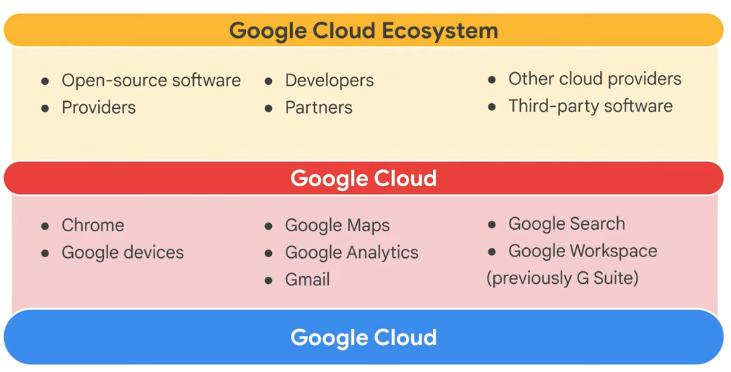
\includegraphics[width=\linewidth]{gc-ecosistema.png}
\par\vspace{1mm}
{\scriptsize Se lee de abajo hacia arriba. La franja roja: los productos de Google.}
\column{.47\textwidth}
\begin{block}{Abajo: Google Cloud}
\small Los centros de datos y la red. La \textbf{misma} infraestructura que usa Google para lo suyo.
\end{block}
\begin{block}{Al medio: los productos de Google}
\small Gmail, Maps, Search: corren sobre esa base. Tú alquilas lo que ellos ya usan.
\end{block}
\begin{block}{Arriba: el ecosistema}
\small \textbf{Código abierto} (Linux, Kubernetes), \textbf{socios} que te ayudan a implementar, \textbf{otras nubes} y \textbf{software de terceros} (WordPress, MongoDB).
\end{block}
\end{columns}
\par\vspace{1mm}
\begin{exampleblock}{Una comparación}
\small \textbf{Android}: el sistema es la base; encima, las apps de Google; y arriba, la tienda con las apps de todos.
\end{exampleblock}
\end{frame}

\begin{frame}{Dónde vive Google Cloud: regiones, zonas y red}
\begin{columns}[c,onlytextwidth]
\column{.56\textwidth}
\centering
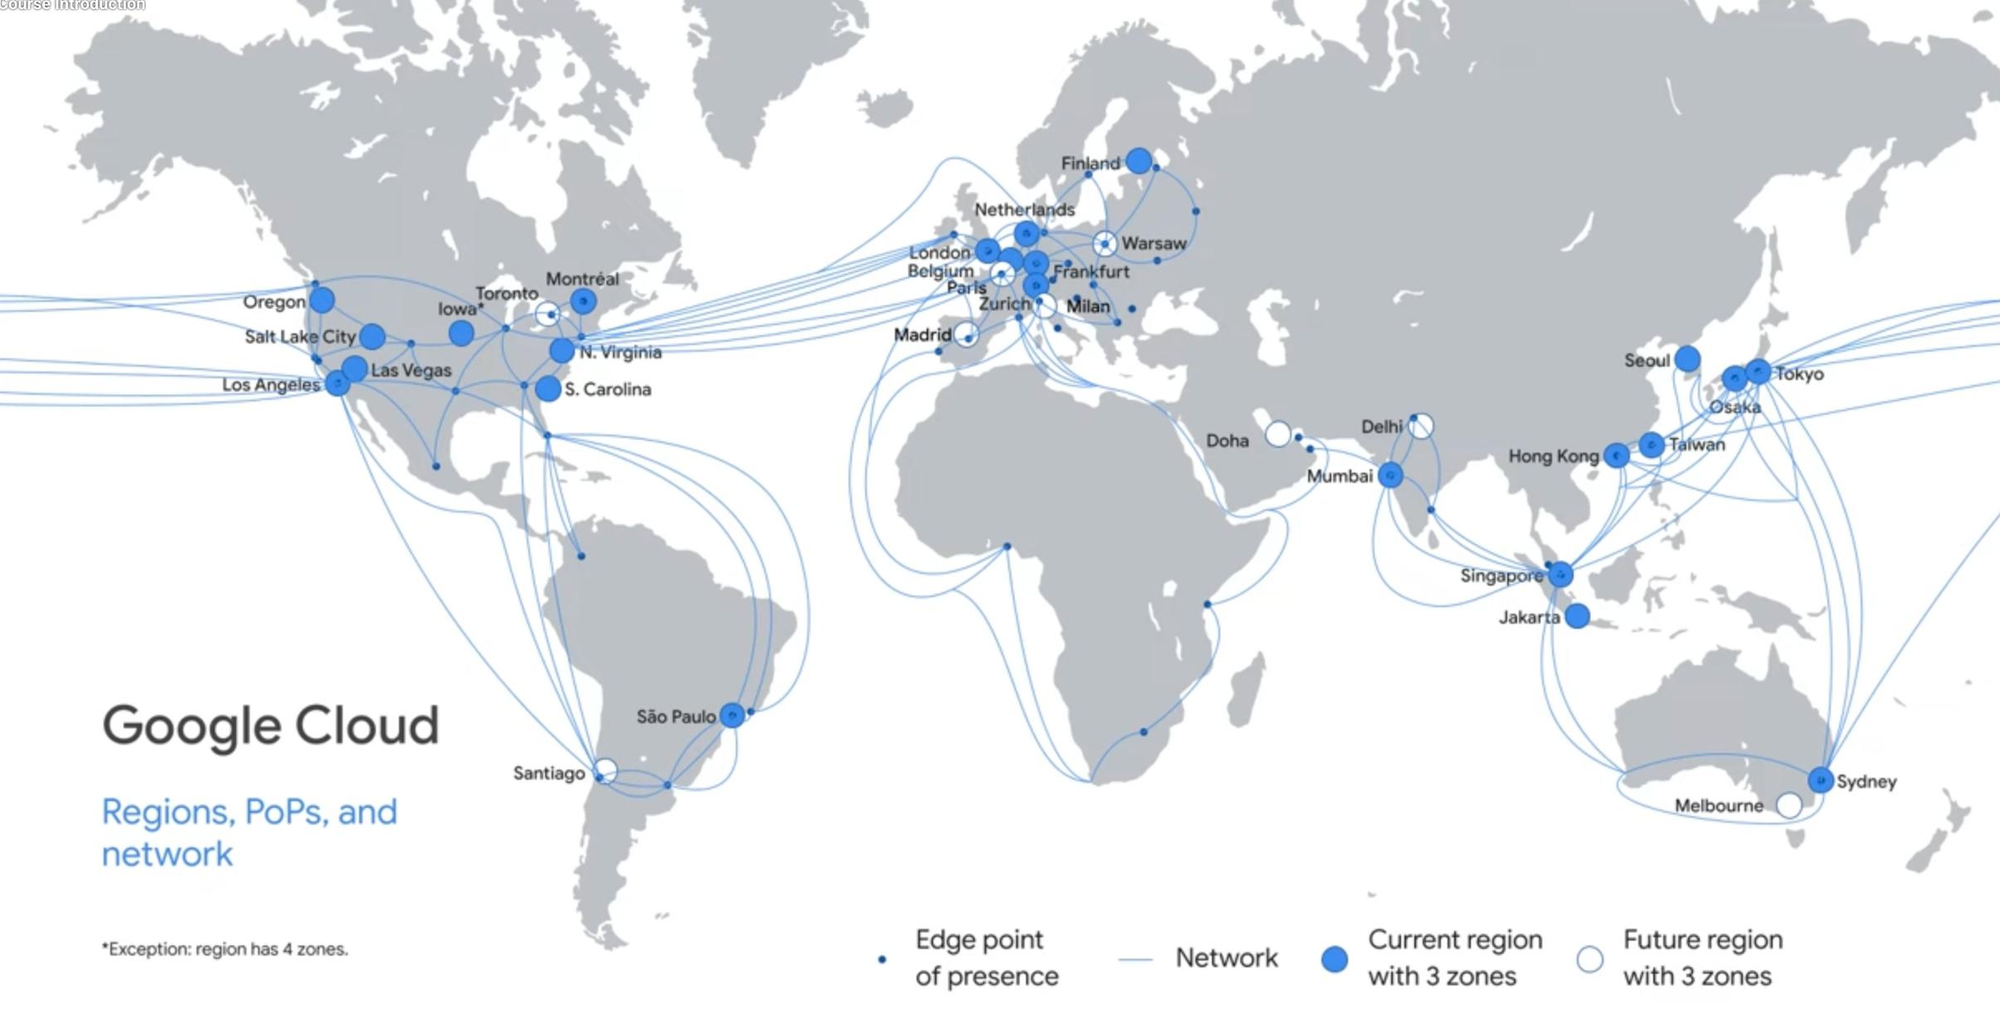
\includegraphics[width=\linewidth]{gc-mapa-regiones.png}
\par\vspace{1mm}
{\scriptsize El mapa es del curso y tiene unos años: Santiago aparece como ``futura'' y ya funciona.}
\column{.42\textwidth}
\begin{block}{Qué significa cada marca}
\footnotesize
\textbf{Región (círculo azul):} un lugar del mundo con centros de datos. Ej.: \texttt{southamerica-west1}, Santiago.\par\smallskip
\textbf{Zona:} un centro de datos independiente dentro de la región. Casi todas tienen \textbf{3}.\par\smallskip
\textbf{Punto de presencia (punto chico):} donde la red de Google se conecta con Internet, cerca de ti. Ahí no corren tus VMs.\par\smallskip
\textbf{Red (líneas):} fibra y cables submarinos propios.
\end{block}
\end{columns}
\par\vspace{1mm}
\begin{columns}[T,onlytextwidth]
\column{.48\textwidth}
\begin{exampleblock}{Una comparación}
\small Un servicio de \textbf{delivery}: la región es la ciudad con almacenes; la zona, cada almacén; el punto de presencia, el punto de recojo de tu barrio.
\end{exampleblock}
\column{.48\textwidth}
\begin{alertblock}{Desde Perú}
\small Las regiones más cercanas son \textbf{Santiago} y \textbf{São Paulo}. Más cerca significa respuestas más rápidas.
\end{alertblock}
\end{columns}
\end{frame}

\begin{frame}{Cinco formas de ejecutar tu programa}
\centering
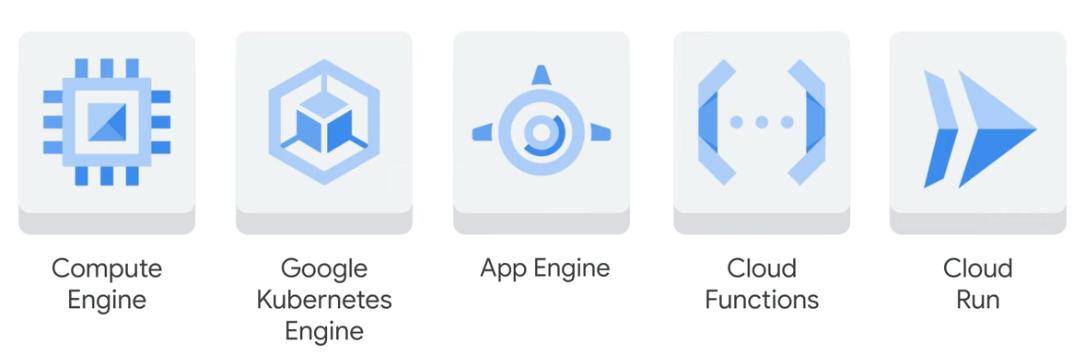
\includegraphics[height=1.75cm]{gc-opciones-computo.png}
\par
\renewcommand{\arraystretch}{1.15}
\footnotesize
\begin{tabular}{@{}p{2.4cm}p{4.2cm}p{3.2cm}p{2.8cm}@{}}
\toprule
\textbf{Servicio} & \textbf{Qué te da} & \textbf{Como\ldots} & \textbf{Fuera de Google}\\
\midrule
Compute Engine & Una VM: tú instalas todo & alquilar una casa vacía & VirtualBox en tu PC\\
Kubernetes Engine & Ordena muchos contenedores & jefe de patio de comidas & minikube en tu PC\\
App Engine & Subes código, sin ver servidores & departamento amoblado & Render\\
Cloud Functions & Una función que corre si pasa algo & luz con sensor & Cloudflare Workers\\
Cloud Run & Tu contenedor; se apaga sin visitas & taxi: pagas el viaje & Render\\
\bottomrule
\end{tabular}
\par\vspace{1mm}
\begin{columns}[T,onlytextwidth]
\column{.48\textwidth}
\begin{exampleblock}{Una palabra nueva}
\footnotesize \textbf{Contenedor:} una caja con tu programa y todo lo que necesita para correr. La herramienta más conocida es Docker.
\end{exampleblock}
\column{.48\textwidth}
\begin{alertblock}{Dos aclaraciones}
\footnotesize \emph{Cloud Functions} hoy se llama \textbf{Cloud Run functions}. Y este curso se queda en \textbf{Compute Engine}.
\end{alertblock}
\end{columns}
\end{frame}

\begin{frame}{Cuatro formas de hablar con Google Cloud}
\begin{columns}[c,onlytextwidth]
\column{.52\textwidth}
\centering
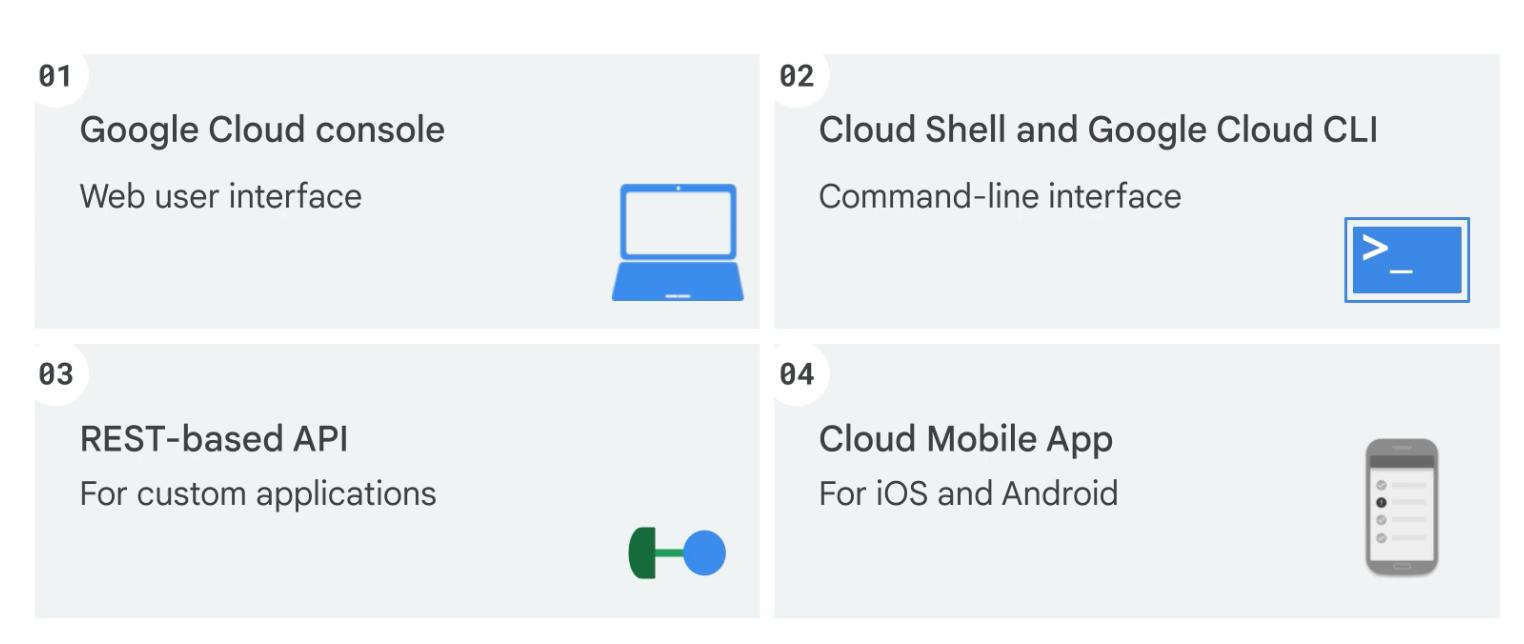
\includegraphics[width=\linewidth]{gc-cuatro-formas.png}
\par\vspace{2mm}
\begin{block}{Tres siglas}
\footnotesize
\textbf{CLI:} interfaz de línea de comandos; escribes texto.\par
\textbf{API:} la forma en que un programa le pide algo a otro.\par
\textbf{REST:} un estilo de API que usa direcciones web, igual que tu navegador.
\end{block}
\column{.45\textwidth}
\renewcommand{\arraystretch}{1.3}
\footnotesize
\begin{tabular}{@{}p{2.3cm}>{\raggedright\arraybackslash}p{3.3cm}@{}}
\toprule
\textbf{Google Cloud} & \textbf{Lo mismo en GitHub}\\
\midrule
1. Consola (web) & la página \texttt{github.com}\\
2. Cloud Shell y \texttt{gcloud} & \texttt{git} y \texttt{gh} en la terminal\\
3. API REST & la API de GitHub que usa tu programa\\
4. App móvil & GitHub Mobile\\
\bottomrule
\end{tabular}
\par\vspace{2mm}
\begin{exampleblock}{Otra comparación}
\small Pedir comida: en el local, por teléfono, con la app, o que el sistema de tu empresa haga el pedido solo.
\end{exampleblock}
\end{columns}
\par\vspace{1mm}
\begin{alertblock}{La idea de fondo}
\small Las cuatro terminan llamando a la \textbf{misma API}. Lo que creas con una, lo ves con las otras.
\end{alertblock}
\end{frame}

\begin{frame}{Forma 1: la consola de Google Cloud}
\centering
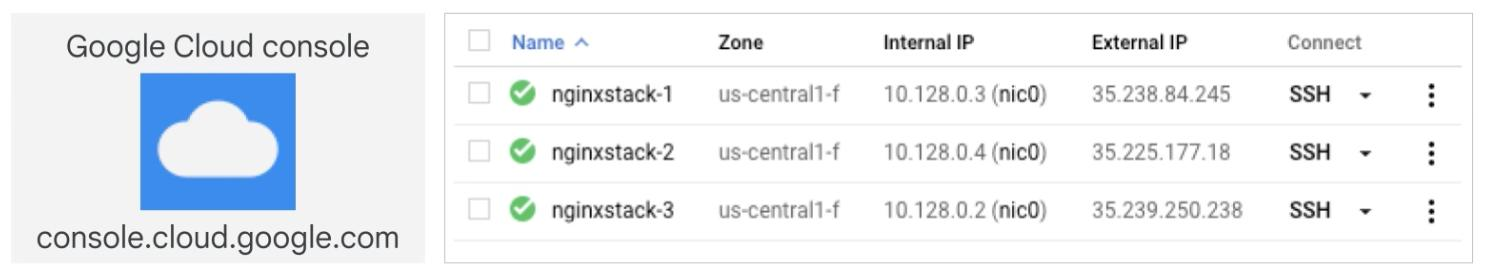
\includegraphics[width=.92\linewidth]{gc-consola.png}
\par\vspace{2mm}
\begin{columns}[T,onlytextwidth]
\column{.48\textwidth}
\begin{block}{Qué es}
\small Una \textbf{página web} (\texttt{console.cloud.google.com}) donde ves y administras todo con clics, menús y formularios.
\end{block}
\begin{exampleblock}{Se parece a}
\small La \textbf{banca por Internet} de tu banco, o el panel de Vercel, Netlify o cPanel donde administras tu sitio.
\end{exampleblock}
\column{.48\textwidth}
\begin{block}{Cómo leer la tabla de la imagen}
\footnotesize
Cada fila es una \textbf{VM} (máquina virtual). El check verde: está \textbf{encendida}.\par\smallskip
\textbf{Zone:} en qué zona vive (\texttt{us-central1-f}).\par
\textbf{Internal IP:} su dirección dentro de la red. \texttt{nic0} es su tarjeta de red.\par
\textbf{External IP:} su dirección en Internet.\par
\textbf{SSH:} botón que abre una terminal \textbf{dentro} de esa VM.
\end{block}
\end{columns}
\end{frame}

\begin{frame}{Forma 2: la CLI de Google Cloud (\texttt{gcloud})}
\centering
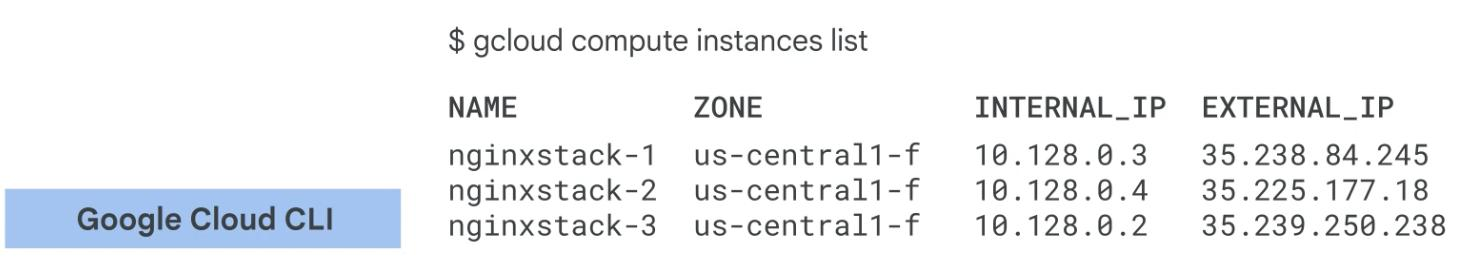
\includegraphics[width=.86\linewidth]{gc-cli.png}
\par\vspace{1mm}
\begin{tikzpicture}[font=\small,
  parte/.style={draw=utpRojo,rounded corners=3pt,minimum height=.8cm,minimum width=2.5cm,align=center}]
  \node[parte,fill=utpRojo!35] (a) at (0,0) {\texttt{gcloud}};
  \node[parte,fill=utpRojo!22] (b) at (3.0,0) {\texttt{compute}};
  \node[parte,fill=utpRojo!12] (c) at (6.0,0) {\texttt{instances}};
  \node[parte,fill=white] (d) at (9.0,0) {\texttt{list}};
  \node[font=\footnotesize,below=1mm of a.south,anchor=north] {el programa};
  \node[font=\footnotesize,below=1mm of b.south,anchor=north] {el servicio};
  \node[font=\footnotesize,below=1mm of c.south,anchor=north] {el recurso (las VMs)};
  \node[font=\footnotesize,below=1mm of d.south,anchor=north] {la acción};
\end{tikzpicture}
\par\vspace{1mm}
\begin{columns}[T,onlytextwidth]
\column{.48\textwidth}
\begin{block}{Qué es}
\small Un programa que se maneja \textbf{escribiendo}. Muestra las \textbf{mismas tres VMs} que la consola, como texto. El \texttt{\$} del inicio no se escribe: solo avisa que la terminal espera.
\end{block}
\column{.48\textwidth}
\begin{exampleblock}{El mismo patrón en otras herramientas}
\small \texttt{git status}, \texttt{docker ps}, \texttt{npm install}: programa, luego qué quieres hacer. En AWS: \texttt{aws ec2 describe-instances}.
\end{exampleblock}
\end{columns}
\end{frame}

\begin{frame}{Cloud Shell: la terminal que ya viene lista}
\begin{columns}[c,onlytextwidth]
\column{.54\textwidth}
\centering
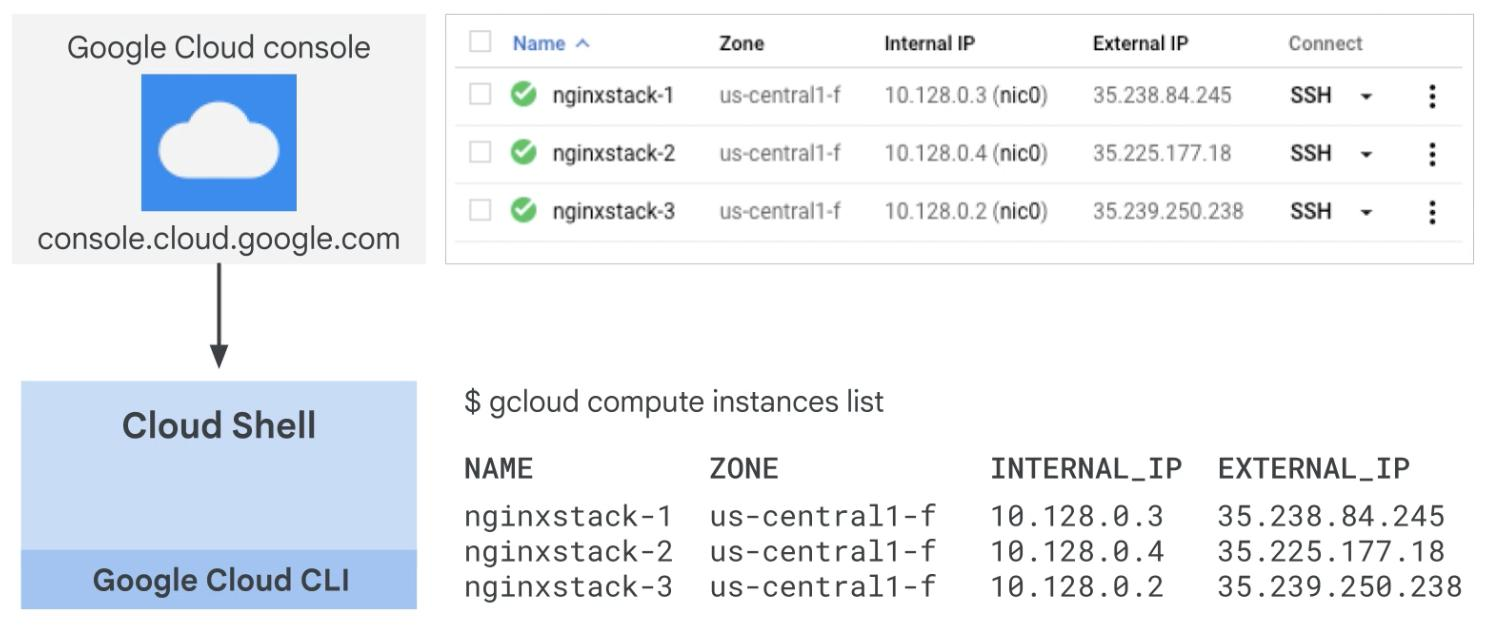
\includegraphics[width=\linewidth]{gc-cloud-shell.png}
\column{.43\textwidth}
\begin{block}{Dos caminos para usar \texttt{gcloud}}
\small
\textbf{En tu laptop:} descargas e instalas la CLI y luego inicias sesión.\par\smallskip
\textbf{En Cloud Shell:} abres la consola, haces clic en un botón y ya está instalada y con tu usuario.
\end{block}
\begin{block}{Qué es Cloud Shell}
\small Una computadora Linux \textbf{prestada} que se maneja desde el navegador. La flecha de la imagen dice eso: se abre \textbf{desde} la consola.
\end{block}
\end{columns}
\par\vspace{1mm}
\begin{columns}[T,onlytextwidth]
\column{.48\textwidth}
\begin{exampleblock}{Una comparación}
\small \textbf{Google Docs} frente a instalar Word: abres el navegador y escribes, sin instalar nada.
\end{exampleblock}
\column{.48\textwidth}
\begin{alertblock}{Lo mismo, fuera de Google}
\small \textbf{GitHub Codespaces} y \textbf{Replit} (con plan gratuito). AWS y Azure tienen su propio CloudShell.
\end{alertblock}
\end{columns}
\end{frame}

% --------------------------------------------------------------- El lab
\begin{frame}[plain]
\vfill
\begin{center}
{\fontsize{29}{34}\selectfont\bfseries El lab, tarea por tarea}\par
\vspace{2mm}
{\small \emph{Explora la consola de Google Cloud y Cloud Shell}}\par
\vspace{4mm}
{\color{utpRojo}\rule{8.5cm}{1.2pt}}
\end{center}
\vfill
\end{frame}

\begin{frame}{Mapa del lab}
\begin{block}{De qué trata}
\small Haces \textbf{lo mismo de dos maneras}: creas un lugar para guardar archivos con clics y luego con comandos. Después aprendes a que Cloud Shell \textbf{recuerde} tus datos.
\end{block}
\renewcommand{\arraystretch}{1.25}
\centering\small
\begin{tabular}{@{}p{0.7cm}p{5.4cm}p{6.6cm}@{}}
\toprule
\textbf{\#} & \textbf{Tarea} & \textbf{Lo que aprendes}\\
\midrule
1 & Crea un bucket con la consola & Moverte por los menús\\
2 & Accede a Cloud Shell & Qué es y qué botones tiene\\
3 & Crea un bucket con Cloud Shell & Tu primer comando \texttt{gcloud}\\
4 & Explora más funciones & Subir un archivo y copiarlo al bucket\\
5 & Crea un estado persistente & Variables, archivo de configuración y \texttt{.profile}\\
6 & Revisa la interfaz & Cuándo conviene consola y cuándo comandos\\
\bottomrule
\end{tabular}
\par\vspace{2mm}
\begin{alertblock}{Antes de la tarea 1}
\small \textbf{Comenzar lab}, abrir la consola en \textbf{incógnito}, entrar con el usuario temporal y aceptar los términos.
\end{alertblock}
\end{frame}

\begin{frame}{Antes de la tarea 1: ¿qué es un bucket?}
\begin{columns}[T,onlytextwidth]
\column{.48\textwidth}
\begin{block}{Tres palabras}
\small
\textbf{Cloud Storage:} el servicio de Google Cloud para \textbf{guardar archivos}.\par\smallskip
\textbf{Bucket} (``balde''): el recipiente donde van los archivos. Sin bucket no puedes guardar nada.\par\smallskip
\textbf{Objeto:} cada archivo que metes al bucket: una foto, un PDF, un video.
\end{block}
\begin{exampleblock}{Una comparación}
\small Como una carpeta principal de \textbf{Google Drive}, \textbf{Dropbox} o \textbf{MEGA}. La diferencia: está pensado para que lo usen \textbf{programas}, no personas arrastrando archivos.
\end{exampleblock}
\column{.48\textwidth}
\begin{alertblock}{El nombre es único en todo el mundo}
\small Como un correo de Gmail o un usuario de Instagram: si alguien ya lo tiene, no puedes usarlo.\par\smallskip
Solo \textbf{minúsculas}, números y guiones. No se puede cambiar después.\par\smallskip
\textbf{Truco del lab:} usa el \textbf{ID de tu proyecto}; ya es único.
\end{alertblock}
\begin{block}{Lo mismo, fuera de Google}
\small \textbf{Amazon S3} (el original), \textbf{Cloudflare R2} y \textbf{Backblaze B2} (con capa gratuita), y \textbf{MinIO}, que es gratis y corre en tu PC.
\end{block}
\end{columns}
\end{frame}

\begin{frame}{Tarea 1: crea un bucket con la consola}
\begin{columns}[T,onlytextwidth]
\column{.50\textwidth}
\begin{block}{Paso a paso}
\small
\textbf{1.} Abre el \textbf{menú de navegación}: las tres rayas de arriba a la izquierda.\par\smallskip
\textbf{2.} Entra a \textbf{Cloud Storage} y luego a \textbf{Buckets}.\par\smallskip
\textbf{3.} Clic en \textbf{Crear}.\par\smallskip
\textbf{4.} Escribe el \textbf{nombre}. Lo demás queda con sus valores por defecto.\par\smallskip
\textbf{5.} Clic en \textbf{Crear}. Sale el aviso \emph{Se impedirá el acceso público}: clic en \textbf{Confirmar}.
\end{block}
\begin{alertblock}{No olvides}
\small \textbf{Revisar mi progreso}, en la página del lab, para que la tarea quede en verde.
\end{alertblock}
\column{.46\textwidth}
\begin{exampleblock}{¿Qué es ``acceso público''?}
\small Que \textbf{cualquiera} en Internet pueda leer tus archivos. Al confirmar, el bucket queda \textbf{privado}.\par\smallskip
Es el \emph{Restringido} de Drive, frente a \emph{Cualquier persona con el enlace}.
\end{exampleblock}
\begin{block}{Los valores por defecto que no tocamos}
\footnotesize
\textbf{Ubicación:} en qué región se guardan.\par
\textbf{Clase de almacenamiento:} qué tan seguido leerás los archivos; cambia el precio.
\end{block}
\begin{block}{La campana de arriba}
\footnotesize \textbf{Notificaciones:} ahí la consola avisa qué hizo por detrás y si algo falló.
\end{block}
\end{columns}
\end{frame}

\begin{frame}{Tarea 2: qué es Cloud Shell por dentro}
\begin{block}{Definición}
\small Una \textbf{máquina virtual temporal} con Linux que Google te presta gratis y que manejas desde el navegador.
\end{block}
\renewcommand{\arraystretch}{1.22}
\centering\footnotesize
\begin{tabular}{@{}p{4.6cm}p{8.6cm}@{}}
\toprule
\textbf{Lo que ofrece} & \textbf{Qué significa para ti}\\
\midrule
VM temporal de Compute Engine & Se crea cuando la abres y se apaga sola si no la usas\\
Línea de comandos en el navegador & No instalas nada en tu laptop\\
5 GB de disco persistente & Tu carpeta personal (\texttt{\$HOME}) \textbf{se conserva} entre una sesión y otra\\
\texttt{gcloud} y otras herramientas & Ya vienen instaladas: \texttt{git}, \texttt{docker}, \texttt{kubectl} y editores de texto\\
Lenguajes & Java, Go, Python, Node.js, PHP y Ruby, listos para usar\\
Vista previa web & Abres en tu navegador una web que corre dentro de esa VM\\
Autorización integrada & Ya entra con tu usuario: no pide contraseña ni llaves\\
\bottomrule
\end{tabular}
\par\vspace{2mm}
\begin{exampleblock}{Una comparación}
\small La \textbf{cabina de Internet} otra vez: la PC es prestada y se reinicia, pero tu \textbf{USB} (la carpeta personal de 5 GB) te lo llevas y lo vuelves a conectar.
\end{exampleblock}
\end{frame}

\begin{frame}{Tarea 2: abrir Cloud Shell y reconocer sus botones}
\begin{center}
\begin{tikzpicture}[font=\footnotesize,
  boton/.style={draw=black!60,rounded corners=2pt,fill=white,minimum height=.55cm,inner xsep=4pt}]
  \fill[black!85,rounded corners=4pt] (0,0) rectangle (13.2,1.3);
  \fill[utpGrisClaro] (0,1.3) rectangle (13.2,2.1);
  \draw[black!60,rounded corners=4pt] (0,0) rectangle (13.2,2.1);
  \node[anchor=west,font=\small\bfseries] at (0.2,1.7) {Cloud Shell};
  \node[boton] at (6.6,1.7) {Abrir editor};
  \node[boton] at (8.6,1.7) {tres puntos};
  \node[boton] at (10.2,1.7) {minimizar};
  \node[boton] at (11.55,1.7) {ventana};
  \node[boton] at (12.65,1.7) {X};
  \node[anchor=west,text=white,font=\ttfamily\footnotesize] at (0.2,0.85) {Welcome to Cloud Shell! Type "help" to get started.};
  \node[anchor=west,text=white,font=\ttfamily\footnotesize] at (0.2,0.4) {student\_01@cloudshell:\textasciitilde{} (qwiklabs-gcp-01-abc123)\$};
\end{tikzpicture}
\end{center}
\begin{columns}[T,onlytextwidth]
\column{.48\textwidth}
\begin{block}{Cómo se abre}
\small Clic en el ícono \textbf{Activar Cloud Shell} (arriba a la derecha de la consola), luego \textbf{Continuar} y \textbf{Autorizar}.
\end{block}
\begin{block}{Los botones}
\footnotesize
\textbf{Abrir editor:} un editor de código en el navegador.\par
\textbf{Tres puntos:} subir, descargar y reiniciar.\par
\textbf{Minimizar y ventana nueva:} acomodan el panel.\par
\textbf{X:} cierra la sesión.
\end{block}
\column{.48\textwidth}
\begin{exampleblock}{Cómo leer la última línea (el \emph{prompt})}
\small
\texttt{student\_01}: tu usuario.\par
\texttt{cloudshell}: el nombre de la máquina.\par
\texttt{\textasciitilde}: la carpeta donde estás; ese signo es tu carpeta personal.\par
\texttt{(qwiklabs-gcp-...)}: el proyecto activo.\par
\texttt{\$}: ``te escucho, escribe''.
\end{exampleblock}
\end{columns}
\end{frame}

\begin{frame}[fragile]{Vocabulario mínimo de terminal}
\begin{columns}[T,onlytextwidth]
\column{.48\textwidth}
\begin{block}{Las palabras}
\small
\textbf{Terminal:} la ventana donde escribes.\par
\textbf{Shell:} el programa que entiende lo que escribes. En Cloud Shell es \textbf{Bash}.\par
\textbf{Comando:} una orden. Se ejecuta al presionar \textbf{Enter}.\par
\textbf{Directorio:} una carpeta.\par
\textbf{\texttt{\$HOME} o \texttt{\textasciitilde}:} tu carpeta personal.
\end{block}
\begin{exampleblock}{Una comparación}
\small Un \textbf{chat} con la computadora: escribes un mensaje, ella responde debajo.
\end{exampleblock}
\column{.48\textwidth}
\begin{block}{Cuatro comandos que no rompen nada}
\begin{lstlisting}[basicstyle=\ttfamily\footnotesize]
pwd      # en que carpeta estoy
ls       # que hay aqui
ls -a    # lo mismo, con los ocultos
cat a.txt  # muestra el archivo a.txt
\end{lstlisting}
\end{block}
\begin{alertblock}{Para practicar fuera del lab (gratis)}
\small La Terminal de macOS o Linux; en Windows, \textbf{Git Bash} o \textbf{WSL}.
\end{alertblock}
\end{columns}
\begin{block}{Dos reglas}
\small Mayúsculas y minúsculas \textbf{no son lo mismo}. Y la tecla \textbf{Tab} completa los nombres por ti.
\end{block}
\end{frame}

\begin{frame}[fragile]{Tarea 3: crea un bucket con Cloud Shell}
\begin{block}{El comando}
\begin{lstlisting}
gcloud storage buckets create gs://NOMBRE_DE_TU_BUCKET
\end{lstlisting}
\end{block}
\begin{center}
\begin{tikzpicture}[font=\footnotesize,
  parte/.style={draw=utpRojo,rounded corners=3pt,minimum height=.55cm,minimum width=2.3cm,align=center}]
  \node[parte,fill=utpRojo!35] (a) at (0,0) {\texttt{gcloud}};
  \node[parte,fill=utpRojo!25] (b) at (2.6,0) {\texttt{storage}};
  \node[parte,fill=utpRojo!15] (c) at (5.2,0) {\texttt{buckets}};
  \node[parte,fill=utpRojo!8] (d) at (7.8,0) {\texttt{create}};
  \node[parte,fill=white,minimum width=3.0cm] (e) at (10.8,0) {\texttt{gs://nombre}};
  \node[below=1mm of a.south,anchor=north] {programa};
  \node[below=1mm of b.south,anchor=north] {servicio};
  \node[below=1mm of c.south,anchor=north] {recurso};
  \node[below=1mm of d.south,anchor=north] {acción};
  \node[below=1mm of e.south,anchor=north] {a qué};
\end{tikzpicture}
\end{center}
\begin{columns}[T,onlytextwidth]
\column{.48\textwidth}
\begin{exampleblock}{¿Qué es \texttt{gs://}?}
\small Avisa ``esto está en Cloud Storage'', igual que \texttt{https://} avisa ``esto es una página web''.
\end{exampleblock}
\begin{alertblock}{Error típico}
\small Copiar los corchetes: \texttt{gs://[BUCKET\_NAME]}. Solo marcan lo que debes reemplazar.
\end{alertblock}
\column{.48\textwidth}
\begin{block}{Comprueba en la consola}
\small \textbf{Cloud Storage} $\rightarrow$ \textbf{Buckets} $\rightarrow$ \textbf{Actualizar}. Ahora hay \textbf{dos}: el de los clics y el del comando.
\end{block}
\begin{block}{En otros lados}
\footnotesize En AWS: \texttt{aws s3 mb s3://nombre}. En guías antiguas de Google verás \texttt{gsutil mb}; hace lo mismo.
\end{block}
\end{columns}
\end{frame}

\begin{frame}[fragile]{Tarea 4: sube un archivo y cópialo al bucket}
\begin{center}
\begin{tikzpicture}[font=\small,
  caja/.style={draw=utpRojo,rounded corners=4pt,minimum width=3.2cm,minimum height=1.1cm,align=center}]
  \node[caja,fill=white] (l) at (0,0) {\textbf{Tu laptop}\\\footnotesize foto.png};
  \node[caja,fill=utpRojo!12] (s) at (5.2,0) {\textbf{Cloud Shell}\\\footnotesize carpeta personal};
  \node[caja,fill=utpRojo!30] (b) at (10.4,0) {\textbf{Bucket}\\\footnotesize Cloud Storage};
  \draw[-latex,thick] (l) -- node[above,font=\footnotesize] {1. Subir} (s);
  \draw[-latex,thick] (s) -- node[above,font=\footnotesize] {2. \texttt{cp}} (b);
\end{tikzpicture}
\end{center}
\begin{columns}[T,onlytextwidth]
\column{.48\textwidth}
\begin{block}{Salto 1: de tu laptop a Cloud Shell}
\small En la barra de Cloud Shell: \textbf{tres puntos} $\rightarrow$ \textbf{Subir}. Elige cualquier archivo. Llega a tu carpeta personal; compruébalo con \texttt{ls}.
\end{block}
\begin{exampleblock}{Una comparación}
\small Pasas la foto del celular a la PC de la cabina, y recién de ahí a tu Drive. Son \textbf{dos lugares distintos}.
\end{exampleblock}
\column{.48\textwidth}
\begin{block}{Salto 2: de Cloud Shell al bucket}
\begin{lstlisting}[basicstyle=\ttfamily\footnotesize]
gcloud storage cp foto.png gs://NOMBRE
\end{lstlisting}
\small \texttt{cp} es \emph{copy}: primero \textbf{qué} copias, después \textbf{a dónde}.
\end{block}
\begin{alertblock}{Si dice que no encuentra el archivo}
\small El nombre no está igual. Escribe las primeras letras y presiona \textbf{Tab}.
\end{alertblock}
\end{columns}
\end{frame}

\begin{frame}[fragile]{Tarea 5 (a): guardar un dato en una variable}
\begin{columns}[T,onlytextwidth]
\column{.50\textwidth}
\begin{block}{Los comandos}
\begin{lstlisting}[basicstyle=\ttfamily\footnotesize]
gcloud compute regions list
INFRACLASS_REGION=us-central1
echo $INFRACLASS_REGION
\end{lstlisting}
\end{block}
\begin{block}{Línea por línea}
\small
\textbf{1.} Lista las regiones disponibles. Eliges una.\par\smallskip
\textbf{2.} Crea la variable y le guarda el valor.\par\smallskip
\textbf{3.} \texttt{echo} \textbf{muestra} un texto; el \texttt{\$} significa ``dame lo que hay dentro de''.
\end{block}
\column{.46\textwidth}
\begin{exampleblock}{¿Qué es una variable de entorno?}
\small Un \textbf{nombre} que guarda un \textbf{valor} mientras dure la sesión.\par\smallskip
Como un \textbf{contacto} del celular: guardas ``Mamá'' y no vuelves a memorizar el número.
\end{exampleblock}
\begin{alertblock}{Errores típicos}
\small Poner \textbf{espacios} alrededor del \texttt{=}.\par
Olvidar el \texttt{\$} al leerla: \texttt{echo} mostraría el nombre, no el valor.
\end{alertblock}
\begin{block}{Ya lo viste antes}
\footnotesize Los archivos \texttt{.env} de un proyecto de Node.js o Python son la misma idea.
\end{block}
\end{columns}
\end{frame}

\begin{frame}[fragile]{Tarea 5 (b): anotar las variables en un archivo}
\begin{block}{Los comandos}
\begin{lstlisting}[basicstyle=\ttfamily\footnotesize]
mkdir infraclass
touch infraclass/config
echo INFRACLASS_REGION=$INFRACLASS_REGION >> ~/infraclass/config
INFRACLASS_PROJECT_ID=el-id-de-tu-proyecto
echo INFRACLASS_PROJECT_ID=$INFRACLASS_PROJECT_ID >> ~/infraclass/config
source infraclass/config
echo $INFRACLASS_PROJECT_ID
\end{lstlisting}
\end{block}
\begin{columns}[T,onlytextwidth]
\column{.48\textwidth}
\begin{block}{Qué hace cada palabra}
\small
\texttt{mkdir}: crea una \textbf{carpeta}.\par
\texttt{touch}: crea un \textbf{archivo vacío}.\par
\texttt{>>}: manda el texto al \textbf{final} de un archivo.\par
\texttt{source}: lee el archivo y \textbf{ejecuta} sus líneas.\par
\texttt{cat infraclass/config}: muestra lo guardado.
\end{block}
\column{.48\textwidth}
\begin{exampleblock}{Una comparación}
\small La variable es algo que tienes \textbf{en la cabeza}; el archivo es \textbf{un papel}. \texttt{source} es volver a leer el papel.
\end{exampleblock}
\begin{alertblock}{Cuidado}
\small Con un solo \texttt{>} se \textbf{borra} lo que había. Con \texttt{>>} se agrega.
\end{alertblock}
\end{columns}
\end{frame}

\begin{frame}[fragile]{Tarea 5 (c): que Cloud Shell lo recuerde solo}
\begin{columns}[T,onlytextwidth]
\column{.48\textwidth}
\begin{alertblock}{El experimento}
\small Cierra Cloud Shell, ábrelo otra vez y escribe \texttt{echo \$INFRACLASS\_PROJECT\_ID}. Sale \textbf{vacío}.\par\smallskip
El archivo sigue en el disco, pero \textbf{nadie lo leyó} en la sesión nueva.
\end{alertblock}
\begin{block}{La solución}
\begin{lstlisting}[basicstyle=\ttfamily\footnotesize]
nano .profile
\end{lstlisting}
\small Al final del archivo agrega:
\begin{lstlisting}[basicstyle=\ttfamily\footnotesize]
source infraclass/config
\end{lstlisting}
\small Guarda con \textbf{Ctrl+O} y \textbf{Enter}; sal con \textbf{Ctrl+X}. Cierra, abre y prueba: ahora \textbf{sí} aparece.
\end{block}
\column{.48\textwidth}
\begin{exampleblock}{Dos definiciones}
\small
\texttt{.profile}: archivo \textbf{oculto} (empieza con punto) que Bash lee \textbf{cada vez} que inicias sesión.\par\smallskip
\texttt{nano}: un editor de texto que funciona dentro de la terminal.
\end{exampleblock}
\begin{block}{Una comparación}
\small \texttt{.profile} es la lista de \textbf{programas de inicio} de Windows: lo que pongas ahí arranca solo.
\end{block}
\renewcommand{\arraystretch}{1.15}
\footnotesize
\begin{tabular}{@{}p{4.0cm}p{2.0cm}@{}}
\toprule
\textbf{Al cerrar Cloud Shell\ldots} & \textbf{¿Sobrevive?}\\
\midrule
Archivos en tu carpeta personal & \textbf{Sí}\\
Variables de la sesión & No\\
Programas instalados fuera de ella & No\\
\bottomrule
\end{tabular}
\end{columns}
\end{frame}

\begin{frame}{Tarea 6: ¿consola o Cloud Shell?}
\renewcommand{\arraystretch}{1.3}
\centering\small
\begin{tabular}{@{}p{2.6cm}p{5.2cm}p{5.2cm}@{}}
\toprule
 & \textbf{Consola (clics)} & \textbf{Cloud Shell (comandos)}\\
\midrule
\textbf{Sirve para} & Ver, explorar, hacer algo por primera vez & Repetir, automatizar, hacer lo mismo cien veces\\
\textbf{Te ayuda con} & Formularios que muestran solo las opciones válidas & Control exacto de cada detalle\\
\textbf{Se guarda como} & Capturas de pantalla & Texto que copias, pegas o conviertes en un \emph{script}\\
\textbf{Su riesgo} & Lento si hay que repetir & Un error de tipeo y falla\\
\bottomrule
\end{tabular}
\par\vspace{3mm}
\begin{columns}[T,onlytextwidth]
\column{.48\textwidth}
\begin{exampleblock}{Una comparación}
\small La consola es pedir con la \textbf{carta con fotos}. Cloud Shell es \textbf{dictarle} el pedido al cocinero: más rápido si ya sabes lo que quieres.
\end{exampleblock}
\column{.48\textwidth}
\begin{alertblock}{No se elige una sola}
\small Se usan \textbf{juntas}. En el lab creaste con comandos y verificaste con clics. Un \emph{script} es un archivo con varios comandos que se ejecutan en orden.
\end{alertblock}
\end{columns}
\end{frame}

\begin{frame}{Errores frecuentes del lab}
\renewcommand{\arraystretch}{1.3}
\centering\small
\begin{tabular}{@{}p{4.6cm}p{4.2cm}p{4.4cm}@{}}
\toprule
\textbf{Lo que ves} & \textbf{Por qué} & \textbf{Qué hacer}\\
\midrule
``El nombre del bucket no está disponible'' & Alguien en el mundo ya lo usa & Usa el ID de tu proyecto\\
``Nombre de bucket no válido'' & Mayúsculas, espacios o corchetes & Solo minúsculas, números y guiones\\
\texttt{command not found} al crear la variable & Hay espacios junto al \texttt{=} & \texttt{NOMBRE=valor}, todo pegado\\
\texttt{echo} muestra una línea vacía & La variable no existe en esta sesión & \texttt{source infraclass/config}\\
\texttt{No such file or directory} & Nombre mal escrito o carpeta sin crear & Revisa con \texttt{ls}; usa Tab\\
La consola abre con tu cuenta personal & No usaste incógnito & Cierra y abre en incógnito\\
\texttt{nano} no guardó el cambio & Saliste sin grabar & Ctrl+O, Enter y recién Ctrl+X\\
\bottomrule
\end{tabular}
\end{frame}

% ------------------------------------------------------------ Practica
\begin{frame}[plain]
\vfill
\begin{center}
{\fontsize{29}{34}\selectfont\bfseries Práctica}\par
\vspace{2mm}
{\small El lab real}\par
\vspace{4mm}
{\color{utpRojo}\rule{8.5cm}{1.2pt}}
\end{center}
\vfill
\end{frame}

\begin{frame}{Práctica: consola y Cloud Shell \textnormal{\small(en clase + tarea)}}
\begin{block}{En clase}
\small
1. Inicia el lab real: \emph{Explora la consola de Google Cloud y Cloud Shell}. Ya sabes qué hace cada comando.\par\smallskip
2. Crea el primer bucket con \textbf{clics} y el segundo con un \textbf{comando}. Fíjate en que los dos aparecen en la consola.\par\smallskip
3. Cierra Cloud Shell, vuelve a abrirlo y comprueba \textbf{qué se conservó} y qué no.
\end{block}
\begin{columns}[T,onlytextwidth]
\column{.48\textwidth}
\begin{exampleblock}{De tarea}
\small Terminar el lab y hacer el curso \emph{Crea una guía de estudio para el examen de la certificación ACE} (1 hora).
\end{exampleblock}
\column{.48\textwidth}
\begin{alertblock}{Entregable}
\small Captura del lab con todas las tareas en verde.
\end{alertblock}
\end{columns}
\end{frame}

\begin{frame}{Cierre: preguntas para comprobar}
\begin{block}{Responde con tus palabras}
\small
1. ¿En qué se diferencian una región, una zona y un punto de presencia?\par\medskip
2. Nombra las cuatro formas de interactuar con Google Cloud. ¿Qué tienen en común?\par\medskip
3. ¿Por qué no pudiste llamar \texttt{fotos} a tu bucket?\par\medskip
4. Explica parte por parte: \texttt{gcloud storage cp foto.png gs://mi-bucket}.\par\medskip
5. Cerraste Cloud Shell. La variable desapareció, pero el archivo \texttt{config} sigue ahí. ¿Por qué? ¿Cómo lo arreglas?\par\medskip
6. Da un caso en que conviene la consola y otro en que conviene Cloud Shell.
\end{block}
\begin{alertblock}{Lo que viene}
\small El segundo lab del módulo: una web completa con \textbf{Marketplace} (pila LAMP), y los labs de \textbf{redes VPC}.
\end{alertblock}
\end{frame}

\begin{frame}[plain]
\begin{tikzpicture}[remember picture,overlay]
  \node[anchor=center,inner sep=0pt] at (current page.center)
    {
\includegraphics[width=\paperwidth,height=\paperheight]{gracias-final.pdf}};
\end{tikzpicture}
\end{frame}

\begin{frame}{Referencias}
\scriptsize
\begin{itemize}\setlength\itemsep{3pt}
  \item Google Skills: ruta \emph{Certificación de Associate Cloud Engineer}, \texttt{skills.google/paths/11}.
  \item Google Skills: \emph{Recorrido por los labs prácticos de Google Cloud} (GSP282).
  \item Google Skills: \emph{Crea una guía de estudio para el examen de la certificación ACE}, \texttt{skills.google/course\_templates/77}.
  \item Google Skills: \emph{Infraestructura esencial de Google Cloud: conceptos básicos}, \texttt{skills.google/course\_templates/50}. Las imágenes del ecosistema, el mapa y las interfaces son de este curso.
  \item Google Skills: lab \emph{Explora la consola de Google Cloud y Cloud Shell}.
  \item Google Cloud: \emph{Cloud Shell documentation}, \texttt{cloud.google.com/shell/docs}.
  \item Google Cloud: \emph{Cloud Storage: buckets} y \emph{gcloud storage}, \texttt{cloud.google.com/storage/docs}.
  \item Google Cloud: \emph{Cloud locations}, \texttt{cloud.google.com/about/locations}.
  \item Material de repaso: \texttt{Sesion16/slides/slides.tex}.
  \item Las respuestas de todas las preguntas de esta sesión están en \texttt{respuestas.md}.
\end{itemize}
\end{frame}

\end{document}
